\documentclass[11pt]{report}
\usepackage{structuralanalysis}
\usepackage{siunitx}
\begin{document}

\begin{tikzpicture}
\point{a}{0}{0};
\point{fprime}{.15}{1}
\point{b}{-.5}{.12};
\point{c}{.5}{.12};
\point{d}{-.5}{.3};
\point{e}{.5}{.3}
\point{f}{0}{1};

\support{3}{a};
\hinge{1}{b}
\hinge{1}{c}
\beam{4}{d}{e}
\beam{4}{d}{f}
\beam{4}{f}{e}
\hinge{1}{f}
\point{g}{6}{1}
\beam{4}{fprime}{g}
\dimensioning{1}{fprime}{g}{2}[\SI{2}{\m}];
%\point{force}{-2}{1.5}
%\load{1}{f}[90]% uncomment to introduce vertical load at the hinge
%\notation{1}{force}{F=10KN}% Just to show the unit and magnitude of the hypothetical force
\end{tikzpicture}
